\chapter{Exemple d'application du langage}
\textcolor{red}{Trouver une manière d'introduire le chapitre}
\section{PlayerUnknown's Battlegrounds (PUBG)\cite{wikipubg}}

PUBG est un jeu vidéo sortit en 2017 avec des millions de joueurs à travers le globe. Développé par PUBG Corporation (filiale de Bluehole, Inc. ou plus récemment de Krafton Game Union) en 2017 c'est un des premiers jeu standalone permettant à ses joueurs de participer à un "last man standing game" suivi de prêt par Fortnite (Epic Games). Ces deux jeux ont été les deux premiers standalone à populariser le Battle Royale et à le mettre à la portée de tous sans devoir développer ou installer des mods dans des jeux existants.

\subsection{L'origine du Battle Royale}
Le Battle Royale trouve ses racines dans le roman Battle Royale et son adaptation cinématographique. Un programme militaire de simulation de combat prend place da ns une République socialiste d'Extrême Orient complètement coupée du monde extérieur sans aucun droits civiques et extrêmement stable politiquement. Le programme consiste à un tirage au sort annuel de 50 classes de troisième qui sont déplacées chacune vers une zone de combat. Au début de l'expérience tous les élèves sont réunis afin d'obtenir un briefing rapide de l'événement et se voient attribuer un sac contenant un objet (allant d'une arme à feu, à une arme blanche, à une fourchette ou une corde de luth). Ils sont ensuite livrés à eux-mêmes dans une zone donnée en ayant pour seule information : aucune règle n'est imposée et un seul survivant par groupe pourra être gagnant de l'expérience les autres devront être exterminés par n'importe quel moyen à disposition. Le champion obtient le droit de vivre aux frais de l'État pour le reste de ses jours et la reconnaissance comme Héros du pays.

\subsection{La naissance de la popularité du Battle Royale}
L'intérêt pour le principe du Battle Royale n'explose que plus tard avec le succès de la saga Hunger Games mettant en place l'histoire de Katniss Everdeen, une jeune adulte qui participe de son plein gré aux Hunger Games. Dans un État totalitaire séparé en castes regroupées dans des districts, deux enfants et/ou adolescents sont choisis au hasard dans chaque district afin de devenir les Tribus. Ils sont alors réunis à la capitale et lâchés dans une arène afin de participer à une télé-réalité de match à mort diffusée partout dans le pays.
Son succès a amené les développeurs du jeu Arma II à créer un mode de jeu basé sur les mêmes règles. Ce mode sera alors appelé DayZ et deviendra par la suite un jeu standalone. Un mode voit également le jour : Battle Royale. Développé par Brendan Greene pour Arma II et ensuite Arma III, ce mode gagne suffisament en popularité pour que celui-ci donne naissance au projet de jeu PlayerUnknown's Battlegrounds (PlayerUnknown étant le pseudonyme en ligne utilisé par Brendan Greene).

\subsection{Les règles de PUBG}
Un avion parcours une ligne droite sur une carte, les 100 joueurs de la partie doivent sauter de cet avion afin d'être parachutés à l'endroit de leur choix à condition qu'il soit à portée. Une fois arrivés au sol, les joueurs partent à la recherche d'armes et d'équipement dans des bâtiments et doivent s'entretuer jusqu'à ce qu'un seul joueur ne soit vivant et gagne ainsi la partie (il est également possible de jouer en duo ou en squad de 4 joueurs ou la dernière équipe debout devient gagnante). Afin de limiter la durée d'une partie, une zone circulaire est définie sur la carte une fois que tous les joueurs ont atterri et celle-ci se réduit par étapes au cours de la partie. Les joueurs en dehors de la zone subissent une certaine quantité de dégâts toutes les secondes s'ils restent en dehors du cercle et ces dégâts augmentent au fur et à mesure que le cercle se resserre.

\subsection{Les Battle Royale dans le monde du jeu vidéo}
Ces dernières années une quantité astronomique de Battle Royale voit le jour dans le jeu vidéo. De Fortnite (Epic Games) à PUBG, en passant par Apex Legends (Respawn Entertainement), Ring of Elysium (Tencent Games) pour ne citer que les plus importants. Des dizaines de jeux voient le jour ou se réinventent afin de coller à la mode des Battle Royale. Les plus grandes licences de FPS (First Personal Shooters) s'alignent également à cette mode, c'est ainsi que voient le jours les modes de jeu Z1BR (H1Z1), Firestorm (Battlefield V), Blackout (Call of Duty Black Ops IV). Mais cette offre répond à une demande phénoménale du public pour ce mode de jeu qui s'impose dans le marché à la même place que le type de jeu MOBA (Multiplayer Online Battle Arena) qui était grand favoris du public depuis une dizaine d'années à travers les jeux League Of Legends ou Dota 2. Avec le temps les Battle Royale tentent de se réinventer et de trouver de nouveaux publics en gardant le principe de Battle Royale mais en apportant d'autres univers. C'est ainsi que naissent Last Tide et son univers aquatique immergé, Fall Guys : Ultimate Knockout et son univers colorés où de petits personnages à la physique étrange se battent pour une couronne, Cuisine Royale, qui était à l'origine une blague de développeurs mais qui a rencontré un succès, dans lequel les personnages se battent à l'aide d'ustensiles de cuisine.

\section{Représentation d'une partie des mécaniques de PUBG}
\subsection{Les données}
Données difficiles à obtenir de façon fiable.
Informatiosn extraites de https://pubg.gamepedia.com/
Wikipedia régulièrement mis a jours
Extraction des informations via les fichiers de jeu minés


\subsection{Le profile}
Arbre des stereotypes découpé avec explications
\begin{figure}[H]
    \centering
    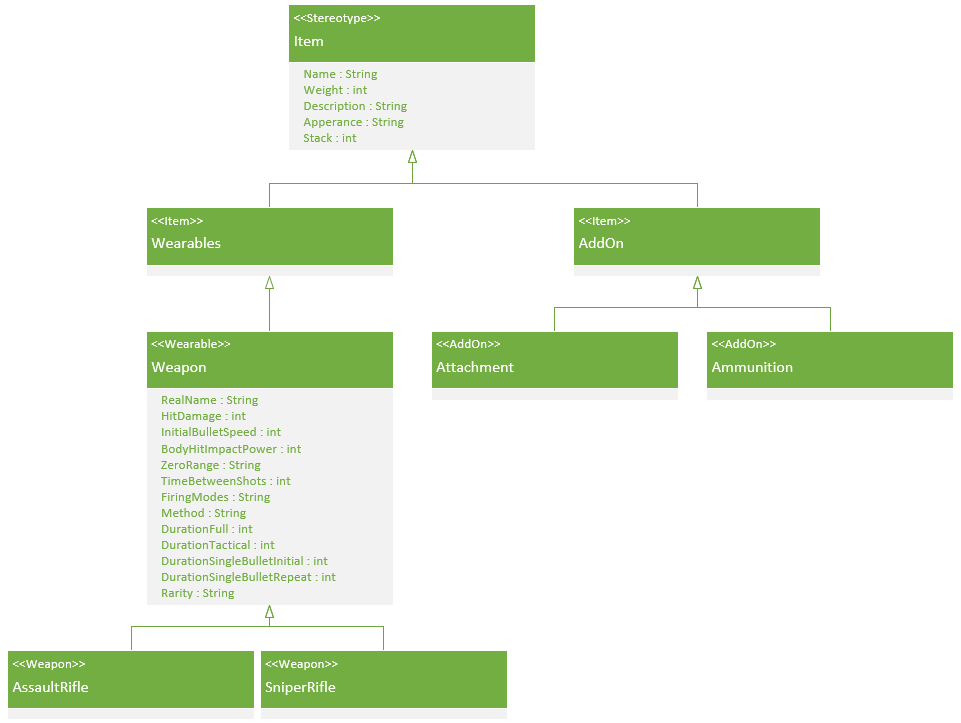
\includegraphics[width=14cm]{10_img/chap6/root(stereotypes).PNG} 
    \caption{Racine des stéréotypes concernés par l'exemple}
\end{figure}
Focus sur la section concernée par la partie decrite plus bas (attachments)



\subsection{La modélisation}

\begin{figure}[H]
    \centering
    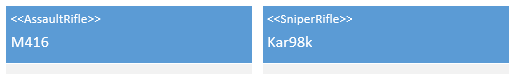
\includegraphics[width=10cm]{10_img/chap6/weapons.PNG} 
    \caption{Classes des "Weapon" concernées par l'exemple}
\end{figure}

\begin{figure}[H]
    \centering
    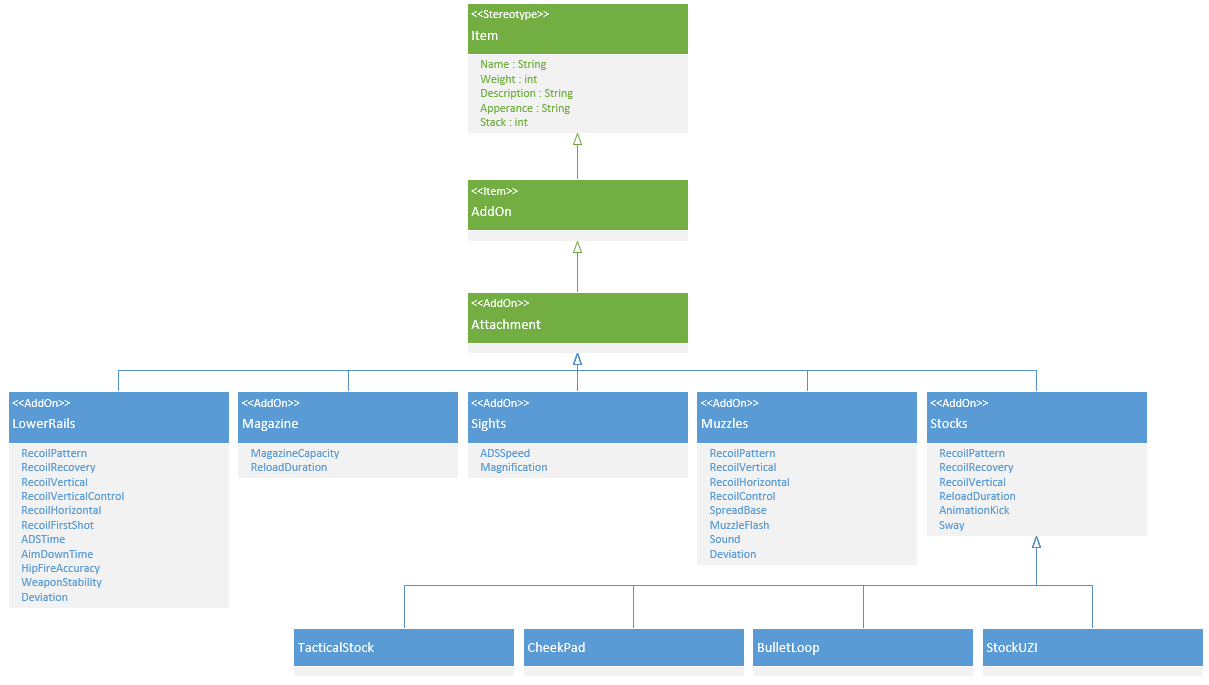
\includegraphics[width=14cm]{10_img/chap6/attachments_stocks.PNG} 
    \caption{Arbre des "Attachment" concernés par l'exemple}
\end{figure}

\begin{figure}[H]
    \centering
    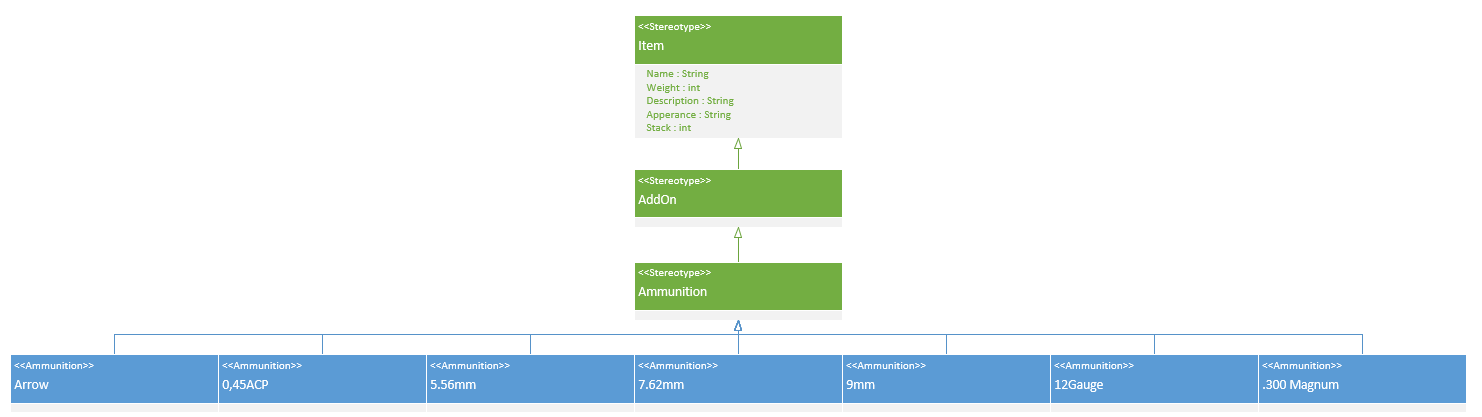
\includegraphics[width=10cm]{10_img/chap6/ammunitions.PNG} 
    \caption{Arbre des "Ammunition" concernés par l'exemple}
\end{figure}


Afin de pouvoir visualiser les interactions entre les éléments il est nécessaire de nommer les associations entre les classes. Afin de mettre en place ces nommages d'associations un groupe de stéréotypes a étét mis en place.


\begin{figure}[H]
    \centering
    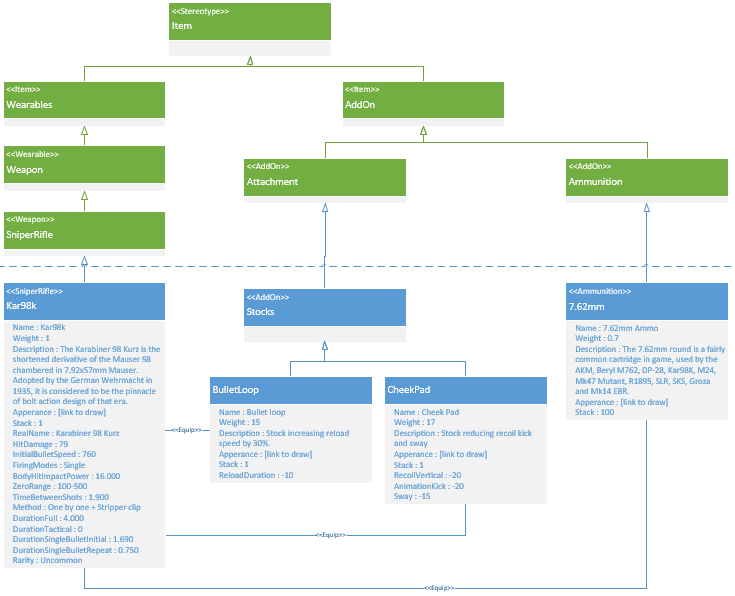
\includegraphics[width=14cm]{10_img/chap6/Kar98k_stock_ammunition_links.PNG} 
    \caption{Arbre du Kar98k, avec ses Stocks et ses Ammunitions concernés par l'exemple}
\end{figure}


\begin{figure}[H]
    \centering
    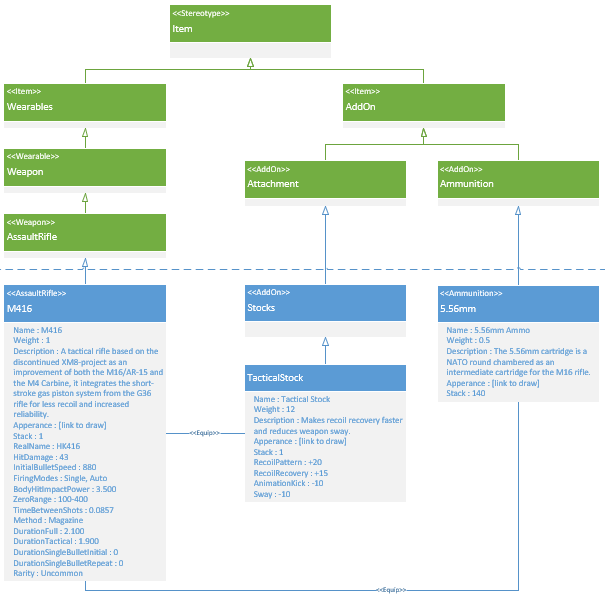
\includegraphics[width=14cm]{10_img/chap6/M416_stock_ammunition_links.PNG} 
    \caption{Arbre du M416, avec ses Stocks et ses Ammunitions concernés par l'exemple}
\end{figure}


\begin{figure}[H]
    \centering
    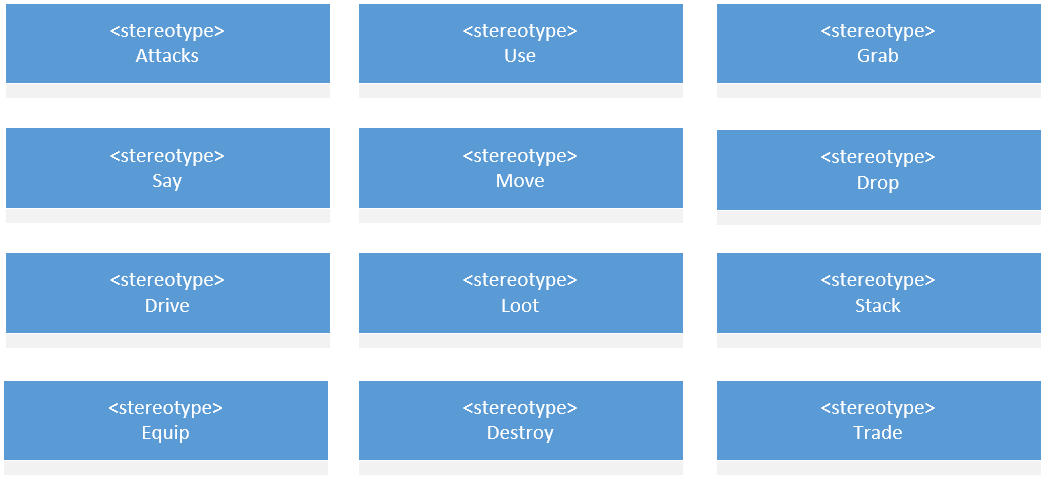
\includegraphics[width=10cm]{10_img/chap6/interacts.PNG} 
    \caption{Arbre des "Interactions" concernées par l'exemple}
\end{figure}

\subsection{Synthèse sous forme de GDD}
Rédaction du GDD avec les informations de la modélisation

\section{Evolutions possibles}
\subsection{Outil de manipulation visuelle du profile UML}
\subsection{Transformation du modèle en GDD}
\subsection{Accélérateur de description des mécaniques}







%%%%%%%%%%%%%%%%%%%%%%%%%%%%%%%%%%%%%%%%%%%%%%%%%%%%%%%%%%%%%%%%%%%%%%%%%%
\begin{comment}
\section{Dans le cadre de Anno1800}
\subsection{Exemple des Mécaniques de Gameplay concernant la Maison d'ouvriers}

\begin{figure}[h!]
    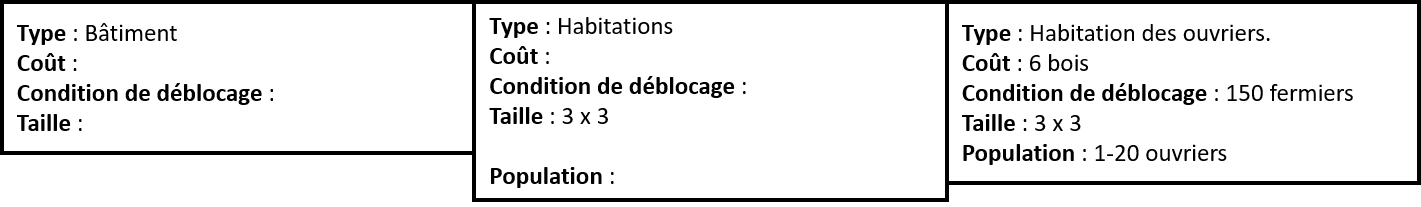
\includegraphics[width=15cm]{10_img/bati_maison_ouvrier.png} 
    \caption{Mécanique de gameplay : Maison d'ouvriers}
\end{figure}

\begin{figure}
    \begin{subfigure}[b]{0.4\textwidth}
        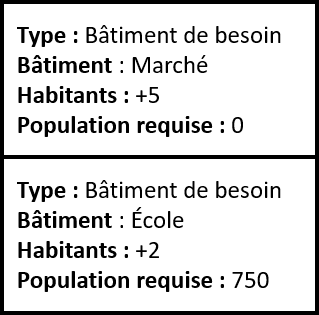
\includegraphics[width=4cm]{10_img/bati_maison_ouvrier_batbesoin.png} 
        \caption{Maison d'ouvriers - Bâtiments de besoins}
    \end{subfigure}
        \hfill
    \begin{subfigure}[b]{0.5\textwidth}
        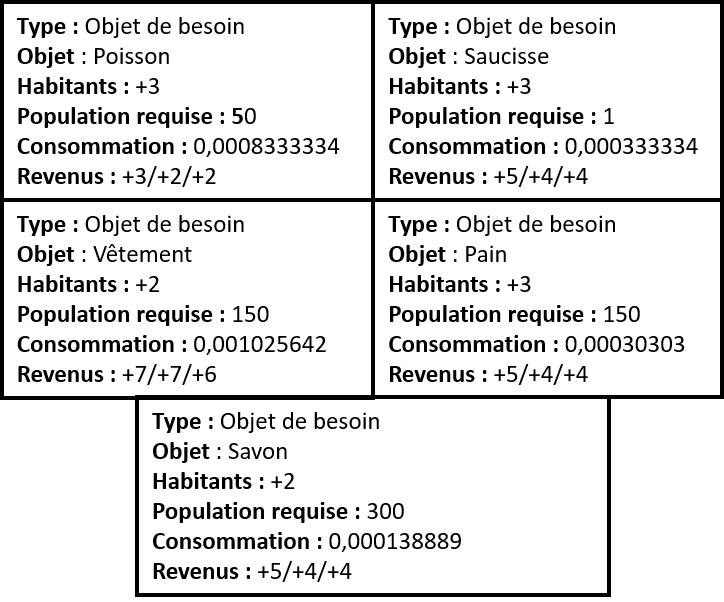
\includegraphics[width=7cm]{10_img/bati_maison_ouvrier_objbesoin.png} 
        \caption{Maison d'ouvriers - Ressources de besoins}
    \end{subfigure}
        \hfill
    \begin{subfigure}[b]{0.4\textwidth}
        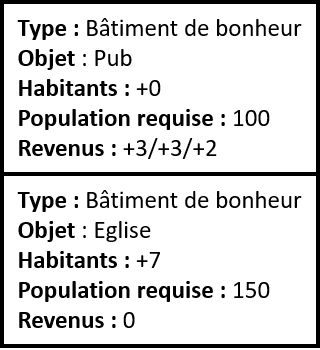
\includegraphics[width=4cm]{10_img/bati_maison_ouvrier_bathonneur.png} 
        \caption{Maison d'ouvriers - Bâtiments de bonheur}
    \end{subfigure}
        \hfill
    \begin{subfigure}[b]{0.4\textwidth}
        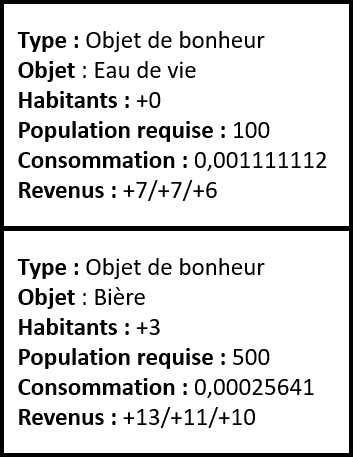
\includegraphics[width=4cm]{10_img/bati_maison_ouvrier_objbonheur.png} 
        \caption{Maison d'ouvriers - Ressources de bonheur}
    \end{subfigure}
    \caption{Mécanique de gameplay : Détails des ressources et bâtiments de besoin et de bonheur}\label{fig:animals}
\end{figure}

\end{comment}
